\section{Introduction - Task 0}

The goal of this assignment is to design and implement a circuit capable of executing \textit{Euclid's algorithm} to compute the \textbf{Greatest Common Divisor (GCD)} for two unsigned integers.

\begin{algorithm}
\caption{Euclid's algorithm for the GCD.}
\begin{algorithmic}
\State \textbf{Input:} $a, b$ integers.
\State \textbf{Output:} GCD of $a$ and $b$.
\State 
\While{$a \neq b$}
    \If{$a > b$}
        \State $a \gets a - b$
    \Else 
        \State $b \gets b - a$
    \EndIf 
\EndWhile
\State \Return $a$
\end{algorithmic}
\end{algorithm}

The assignment specifications require us to design a \textbf{synchronous locally timed (SLT)} module with:
\begin{itemize}
    \item \textbf{Inputs:} a single-bit signal \texttt{req} and a 16-bit unsigned integer \texttt{AB}.
    \item \textbf{Outputs:} a single-bit signal \texttt{ack} and a 16-bit unsigned integer \texttt{C}.  
\end{itemize}

Since the tests will be performed on a Nexys A7 100T FPGA board, the two inputs \texttt{A} and \texttt{B} will be provided through a 2-step \texttt{req-ack} handshake: initially, the first operand is given as input. Then, the second \texttt{req-ack} handshake indicates that the operand is valid and that the computation can start.

The assignment offers a simple implementation using a finite state machine controller and a data-path containing two registers, an ALU, and one multiplexer. 

\begin{figure}[H]
    \centering
    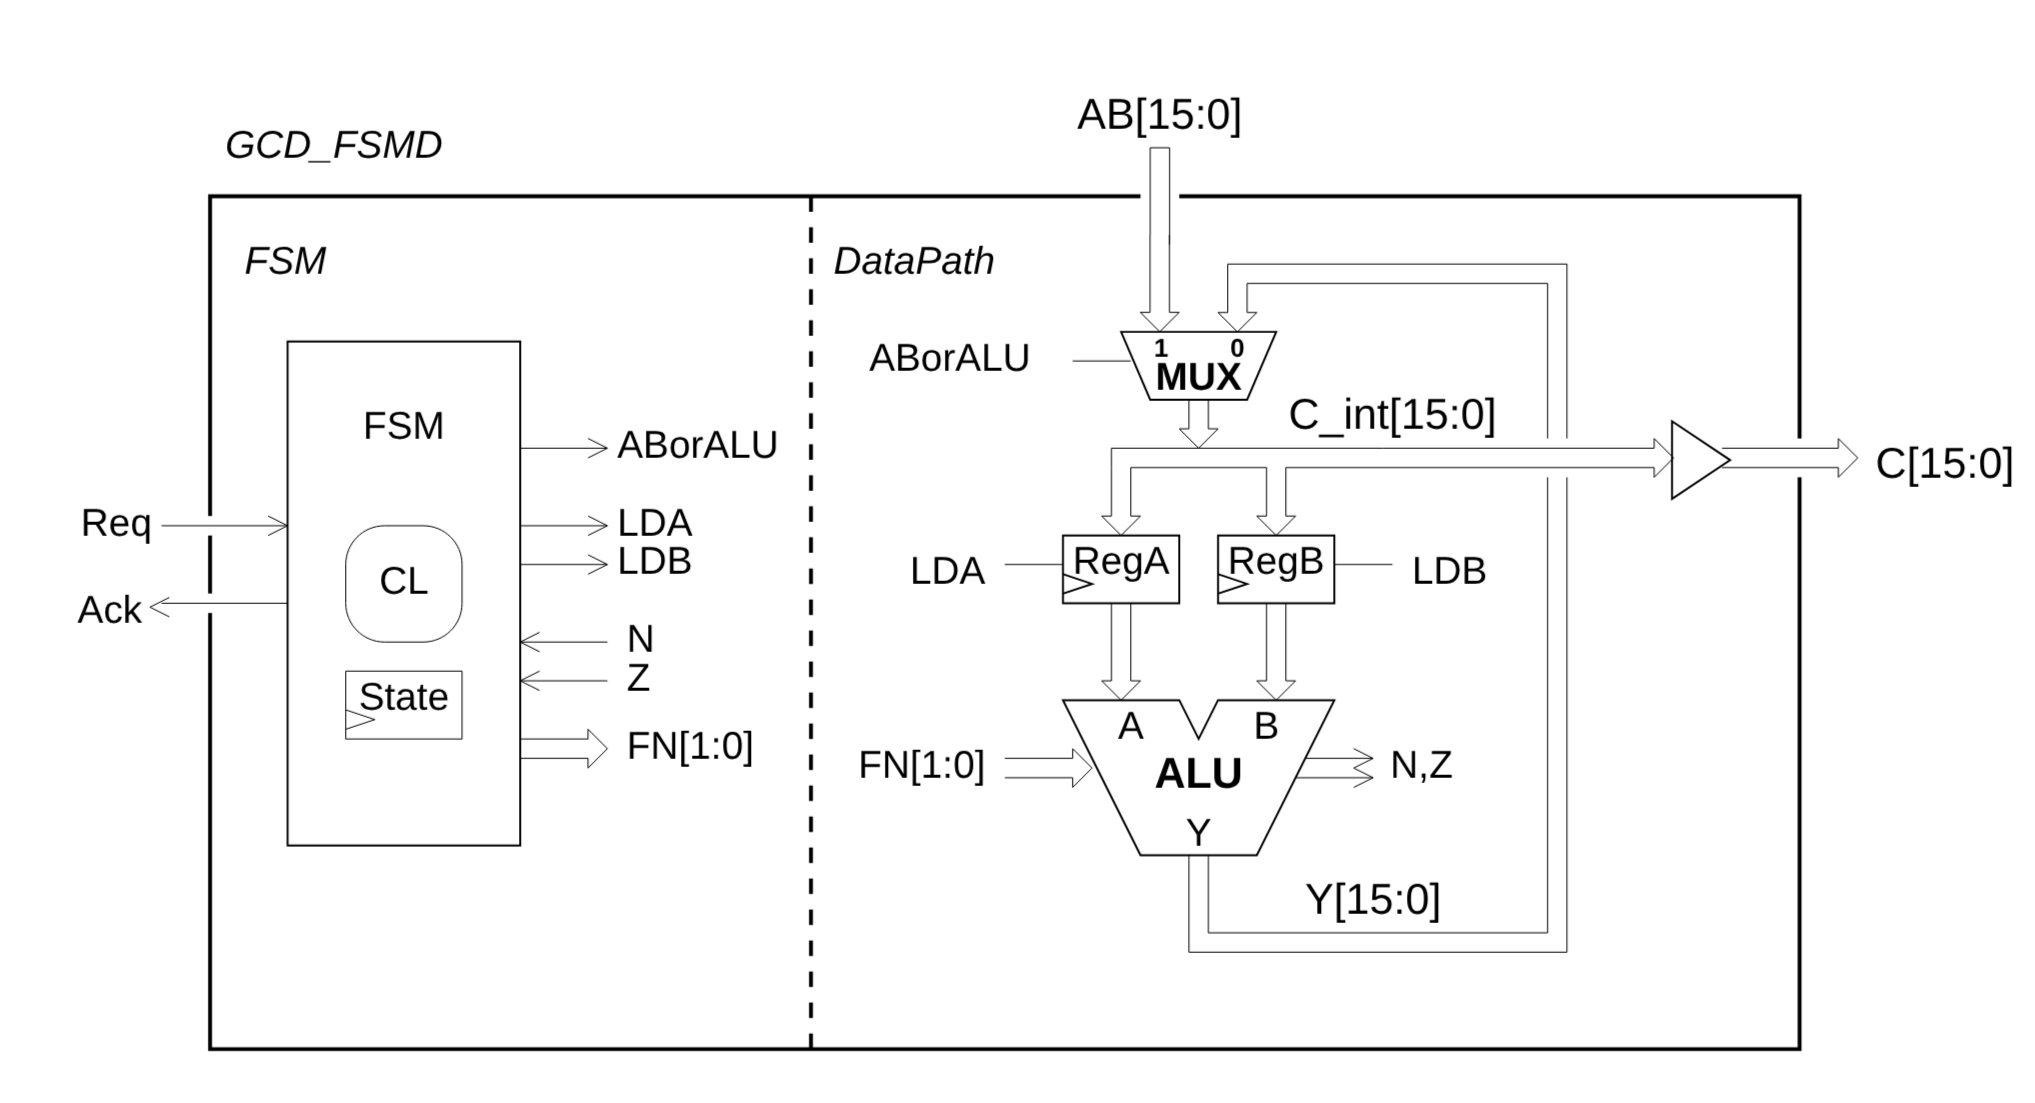
\includegraphics[width=0.85\linewidth]{figures/basic-fsmd-impl.png}
    \caption{FSMD-style implementation of the GCD-module, using two registers
and one ALU.}
    \label{fig:basic-fsmd}
\end{figure}

\begin{table}[H]
\centering
\begin{tabular}{|c|l|l||l|}
\hline
FN[1:0] & \multicolumn{2}{c||}{ALU operation} & Flags (all operations) \\
\hline\hline
00 & subtract & $Y <= A - B$ & $Z <= \text{'1' \text{when} } Y = 0 \text{ (result is zero)}$ \\
01 & subtract & $Y <= B - A$ & $N <= \text{'1' \text{when} } Y[15] = 1 \text{ (result is negative)}$ \\
10 & pass     & $Y <= A$     & \\
11 & pass     & $Y <= B$     & \\
\hline
\end{tabular}
\caption{A possible ALU that could be used in an implementation of the GCD module.}
\label{tab:alu_gcd}
\end{table}

\subsection{Determining the number of LUTs and D-FFs}
\label{resources-estimate}

Let us now assume that the data-path is implemented as shown in Figure \ref{fig:basic-fsmd} and that the technology primitives available on the FPGA board are \textbf{D-flip-flops (D-FFs)} and 6-input \textbf{Look up Tables (LUTs)}. We want to estimate the approximate number of LUTs and D-FFs that will be used to implement the data-path.

Let us first determine the number of D-FFs used in the synthesis: since we require two registers (\texttt{RegA} and \texttt{RegB}), we need 32 flip-flops.

Secondly, to determine the required number of LUTs, we must first take into account that 6-LUTs can implement all boolean functions $\{0,1\}^6\rightarrow \{0,1\}$. Then, let us analyze the data-path block by block:
\begin{itemize}
    \item \textbf{Multiplexer:} the multiplexer outputs a 16-bit unsigned integer; each output bit \texttt{C\_int[i]} is a function of 3 bits (\texttt{AB[i], Y[i], ABOrALU}); thus, 16 LUTs are needed.
    \item \textbf{ALU:} The outputs of the ALU are 18 bits, where the first 16 compute the output value \texttt{Y}. Here we can observe how each bit \texttt{Y[i]} is dependent on 5 input bits (\texttt{A[i], B[i], FN[0], FN[1], carry});\, therefore, no more than 16 LUTs are needed. To compute \texttt{Z}, we can simply use 3 LUTs organized as a cascade of NOR gates. Finally, \texttt{N} can avoid using any LUT, since it can be formulated as \texttt{Y[15]}.
\end{itemize}
In conclusion, we estimate that 32 D-FFs and 35 LUTs are required to build the represented data-path.
